\section{Simulation d'un système de freinage sans ABS}
Durant la pratique des travaux sur VHDL-AMS il est demandé aux étudiants de réaliser et d'instancier étapes par étapes les différentes partie d'un système de freinage d'une voiture. Pour la réalisation du travail nous avons travailler avec le logiciel ModelSim et un éditeur de texte pour venir rédiger, en VHDL, les différentes instances du véhicule jusqu'à l'intégration de l'ABS.

\begin{figure}[h]
    \centering
    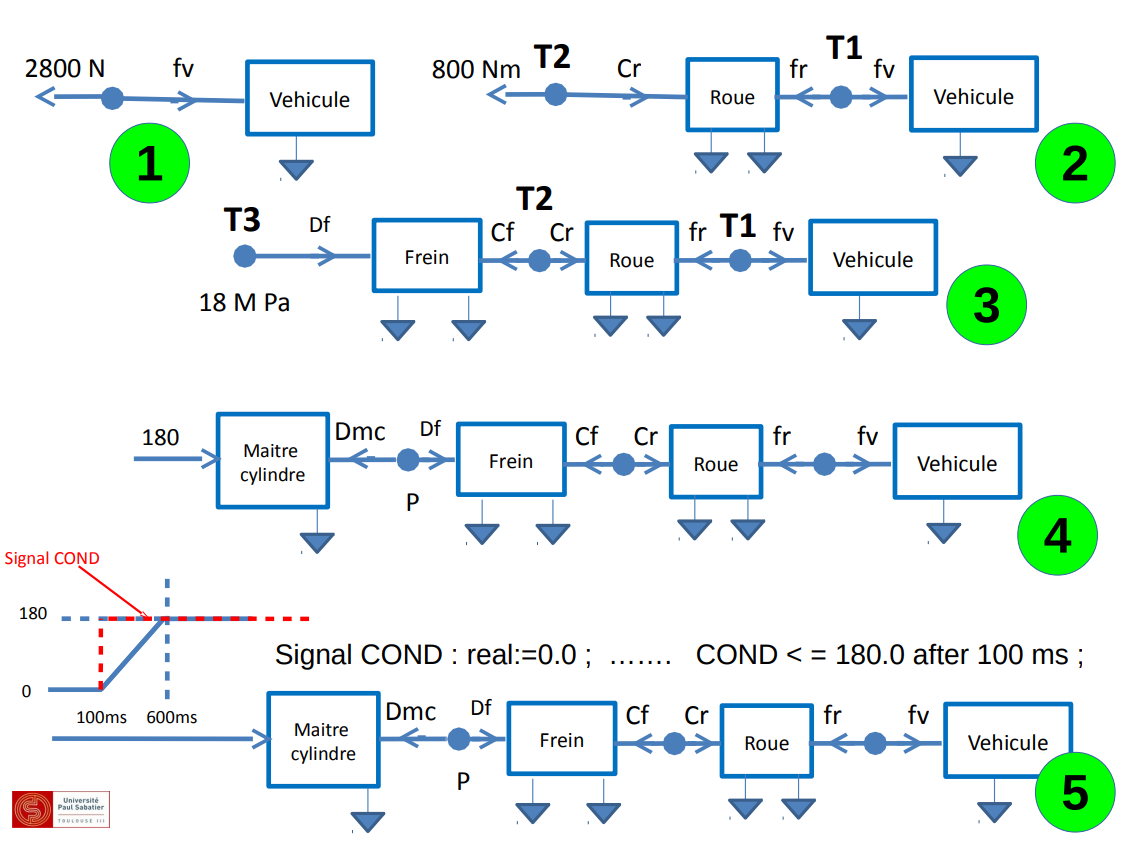
\includegraphics[width=\textwidth]{images/etapes.png}
    \caption{Implémentation des différentes parties du système de freinage d'une voiture}
\end{figure}

Il est demandé d'instancier étapes par étapes différents blocs avec leurs terminaux coresspondants, comme indiqué dans le powerpoint de présentation du TP.

\newpage

\subsection{Analyse instanciation véhicule }
Dans cette première partie nous devons instancier le véhicule fournit dans les fichiers du projet. Sur la Figure 2 on peut voir le schéma bloc qu'il faut instancier son entité en VHDL-AMS.

\begin{figure}[h]
    \centering
    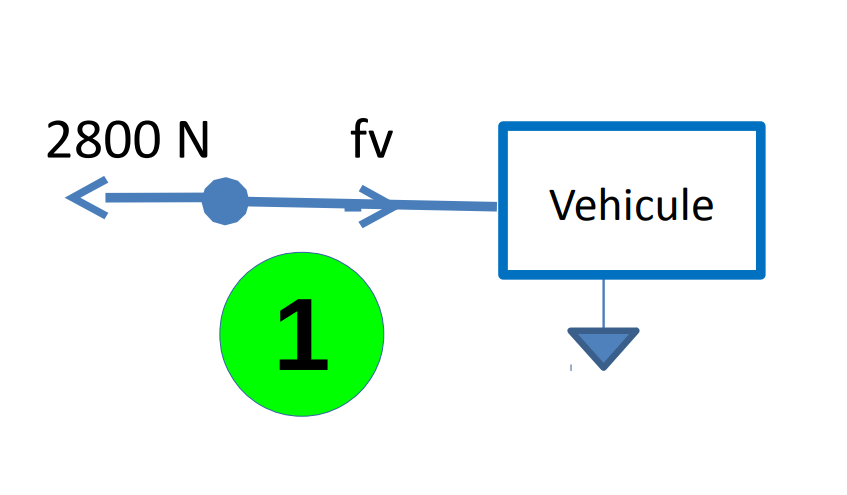
\includegraphics[width=0.5\textwidth]{images/un.png}
    \caption{Instanciation du véhicule avec son terminal}
\end{figure}

Dans l'entité du véhicule nous avons donc à définir certaines quantités qui nous permettra de résoudre certaines équations :\\

\begin{itemize}
        \item $m        \rightarrow$ Masse véhicule.
        \item $Cx       \rightarrow$ Coefficient aérodynamique.
        \item $S        \rightarrow$ Surface Frontale.
        \item $V\_init  \rightarrow$ Vitesse initiale du vehicule.
\end{itemize}

\begin{figure}[h]
    \centering
    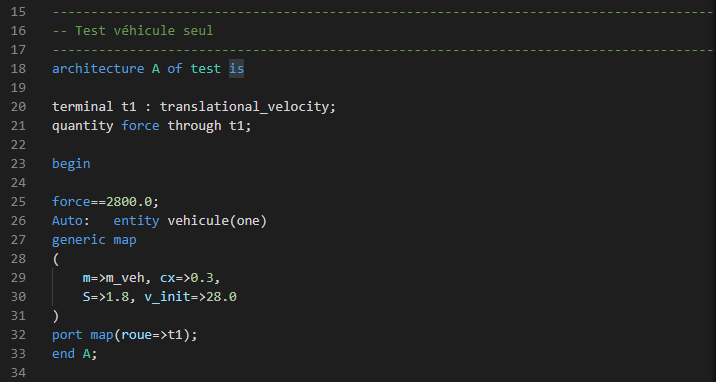
\includegraphics[width=\textwidth]{images/vehicule.png}
    \caption{Code VHDL Architecture A}
\end{figure}

\subsection{Analyse instanciation roue}
a
\subsection{Analyse instanciation frein}
a
\subsection{Analyse instanciation maître cylindre}
a
\subsection{Modélisation du régulateur de pression}
a
\newpage